\documentclass[../docment.tex]{subfiles}
\begin{document}
	\section{这一节重点讲解一下怎么插入图片与表格}
	\subsection{插入图片}
	插入图片就像这个样子,使用命令[]设置的是显示的大小,\{\}中显示的是显示图片的路径,{\heiti 文件名只能是英文字母组成!}
	\begin{figure}
		\centering
		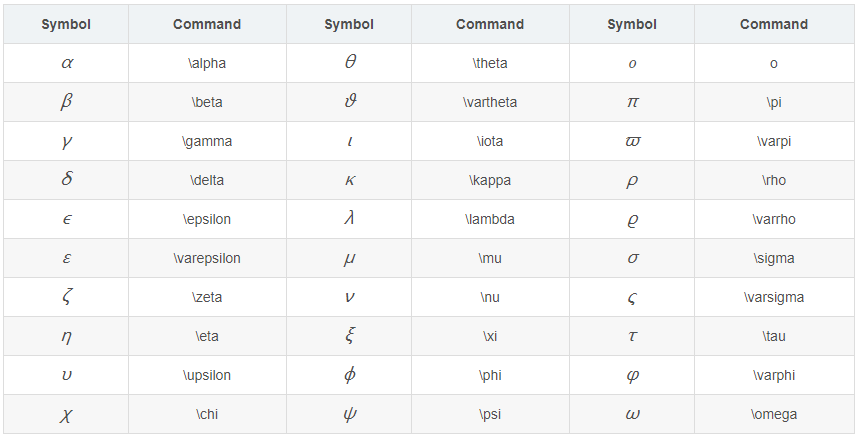
\includegraphics[width=0.50\textheight]{image/image.png}
		\caption{小写希腊字母}
		\label{image:小写希腊字母}
	\end{figure}

	同样的道理,使用$label$做标记,使用$ref$就能够引用,比如你看图(\ref{image:小写希腊字母})就是的。
	
	图片默认显示在当前页面的最上方。
	\subsection{表格}
	插入表格就麻烦多了:
	$ p\{2cm\}<\{ centering \} $表示居中,显示长度为$ 2cm$ , $ caption \{ \}$显示的是表名,$\&$表示的是表中的竖线分割。$hline$显示了横线分割
	这里故意显示了一个超大的表格,给大家看看到底是怎么做的。
	\begin{longtable}{p{2cm}<{\centering} |p{2cm}<{\centering} |p{2.5cm} <{\centering} |p{8cm} }
		\caption{\label{tab:表格}NoSQL和关系数据库的简单比较}  \\
		\hline 
		\hline 
		\textbf{比较标准} 	& \textbf{RDBMS} & \textbf{NoSQL} & \makecell[c]{\textbf{备注}}\\
		\hline
		数据库原理 &完全支持  & 部分支持 & 	RDBMS有关系代数理论作为基础,NoSQL没有统一的理论基础 \\
		\hline
		数据规模 &大  & 超大 & RDBMS很难实现横向扩展,纵向扩展的空间也比较有限,性能会随着数据规模的增大而降低,NoSQL可以很容易通过添加更多设备来支持更大规模的数据 \\
		\hline
		数据库模式 & 固定  & 灵活 & 	RDBMS需要定义数据库模式,严格遵守数据定义和相关约束条	件,NoSQL不存在数据库模式,可以自由灵活定义并存储各种不同类型的数据 \\
		\hline
		查询效率 & 快  & 简单查询快,复杂查询慢 \footnote{可以实现高效的简单查询,但是不具备高度结构化查询等特性,复杂查询的性能不尽人意} & RDBMS借助于索引机制可以实现快速查询(包括记录查询和范围查询),很多NoSQL数据库没有面向复杂查询的索引,虽然NoSQL可以,使用MapReduce来加速查询,但是,在复杂查询方面的性能仍然不如RDBMS \\
		\hline
		一致性 & 强一致性  & 弱一致性 & RDBMS严格遵守事务ACID模型,可以保证事务强一致性,	很多NoSQL数据库放松了对事务ACID四性的要求,而是遵守BASE模型,只能保证最终一致性
		\\
		\hline
		数据完整性 &容易实现  & 很难实现 & 	任何一个RDBMS都可以很容易实现数据完整性,比如通过主键或者非空约束来实现实体完整性,通过主键、外键来实现参照完整性,通过约束或者触发器来实现用户自定义完整性,但是,在NoSQL数据库却无法实现 \\
		\hline
		扩展性 & 一般  & 好 & RDBMS很难实现横向扩展,纵向扩展的空间也比较有限,NoSQL在设计之初就充分考虑了横向扩展的需求,可以很容易通过添加廉价设备实现扩展 \\
		\hline
		可用性 & 好  & 很好 & RDBMS在任何时候都以保证数据一致性为优先目标,其次才是优化系统性能,随着数据规模的增大,RDBMS为了保证严格的一致性,只能提供相对较弱的可用性,大多数NoSQL都能提供较高的可用性 \\
		\hline
		标准化 & 是  & 否 & 	RDBMS已经标准化(SQL)	,NoSQL还没有行业标准,不同的NoSQL数据库都有自己的查询语言,很难规范应用程序接口,StoneBraker认为:NoSQL缺乏统一查询语言,将会拖慢NoSQL发展 \\
		\hline
		技术支持 & 高  & 低 & RDBMS经过几十年的发展,已经非常成熟,Oracle等大型厂商都可以提供很好的技术支持,NoSQL在技术支持方面仍然处于起步阶段,还不成熟,缺乏有力的技术支持
		\\
		\hline
		可维护性 &复杂  & 复杂 & 	RDBMS需要专门的数据库管理员(DBA)维护,NoSQL数据库虽然没有DBMS复杂,也难以维护 \\
		\hline
		\hline
	\end{longtable}
\end{document}